\begin{figure}[thbp]
    \centering
    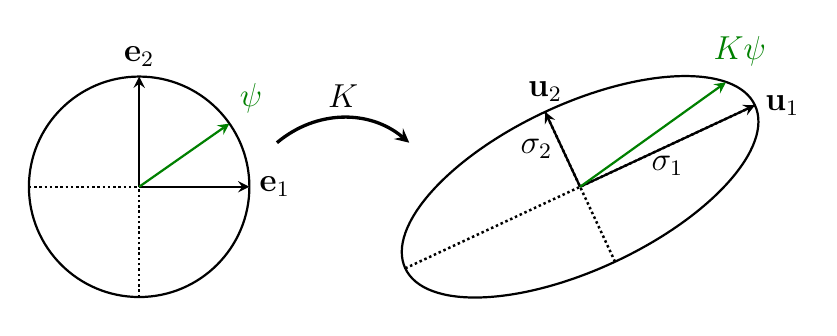
\begin{tikzpicture}[
        scale=0.7,
        >=stealth,
        line width=0.9pt,
        every node/.style={font=\large}
    ]
    % Left: unit circle
    \begin{scope}[shift={(0,0)}]
      % circle
      \draw[thick] (0,0) circle (2);
      % dotted guidelines
      \draw[densely dotted] (-2,0) -- (0,0);
      \draw[densely dotted] (0,-2) -- (0,0);
      % e1, e2
      \draw[thick,->] (0,0) -- (2,0) node[right] {$\mathbf e_1$};
      \draw[thick,->] (0,0) -- (0,2) node[above] {$\mathbf e_2$};
      % omega, length=2, angle=35
      \draw[thick,->,Green] (0,0) -- ({2*cos(35)},{2*sin(35)}) node[above right] {$\boldsymbol{\psi}$};
    \end{scope}
    
    % Middle: K arrow
    \begin{scope}[shift={(3.5,0)}]
      \draw[very thick,->]
        (-1,0.8) to[out=40, in=140] (1.4,0.8);
      \node[above] at (0.2,1.25) {$K$};
    \end{scope}
    
    % Right: ellipse + vectors
    \begin{scope}[shift={(8,0)}, rotate=25]
      % ellipse
      \draw[thick] (0,0) ellipse (3.5 and 1.5);
      % dotted principal axes
      \draw[densely dotted] (-3.5,0) -- (3.5,0);
      \draw[densely dotted] (0,-1.5) -- (0,1.5);
      % u1 and u2
      \draw[thick,->] (0,0) -- (3.5,0)
        node[midway, below] {$\sigma_1$}
        node[right] {$\mathbf u_1$};
      \draw[thick,->] (0,0) -- (0,1.5)
        node[midway, left] {$\sigma_2$}
        node[above] {$\mathbf u_2$};
      % omega
      \draw[thick,->,Green] (0,0) -- (3.2,0.6)
      node[above, xshift=5pt, yshift=2pt] {$K\boldsymbol{\psi}$};
    \end{scope}
    \end{tikzpicture}
    \caption{The geometry of the rSVD. A random sample $K\v\psi$ aligns mostly with the first left singular value. The illustration is inspired by Fig.~9.1 in Tropp \cite{tropp_acm_2021}.}
    \label{fig:rsvd}
\end{figure}